% Created by tikzDevice version 0.12.3.1 on 2022-09-20 08:41:49
% !TEX encoding = UTF-8 Unicode
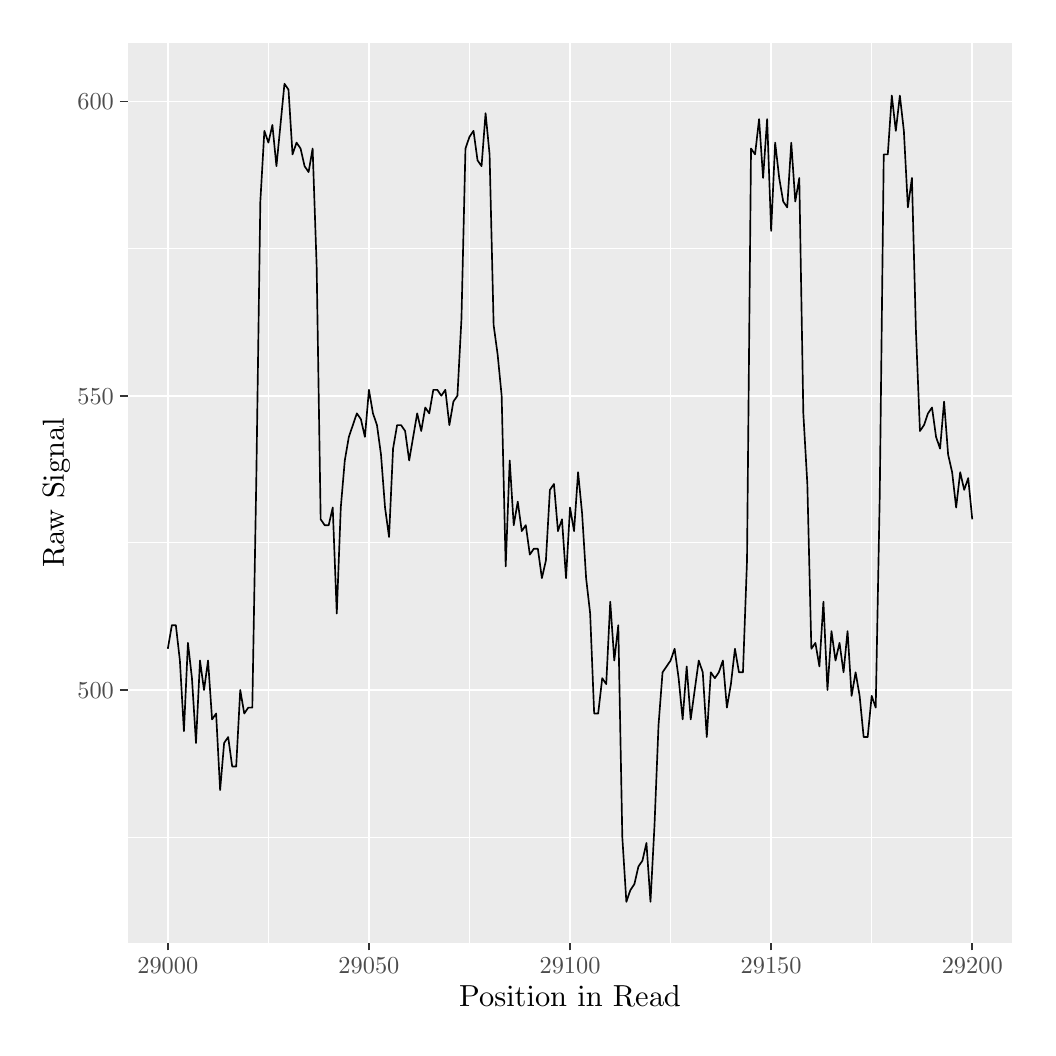
\begin{tikzpicture}[x=1pt,y=1pt]
\definecolor{fillColor}{RGB}{255,255,255}
\path[use as bounding box,fill=fillColor,fill opacity=0.00] (0,0) rectangle (361.35,361.35);
\begin{scope}
\path[clip] (  0.00,  0.00) rectangle (361.35,361.35);
\definecolor{drawColor}{RGB}{255,255,255}
\definecolor{fillColor}{RGB}{255,255,255}

\path[draw=drawColor,line width= 0.6pt,line join=round,line cap=round,fill=fillColor] (  0.00,  0.00) rectangle (361.35,361.35);
\end{scope}
\begin{scope}
\path[clip] ( 36.11, 30.69) rectangle (355.85,355.85);
\definecolor{fillColor}{gray}{0.92}

\path[fill=fillColor] ( 36.11, 30.69) rectangle (355.85,355.85);
\definecolor{drawColor}{RGB}{255,255,255}

\path[draw=drawColor,line width= 0.3pt,line join=round] ( 36.11, 68.86) --
	(355.85, 68.86);

\path[draw=drawColor,line width= 0.3pt,line join=round] ( 36.11,175.19) --
	(355.85,175.19);

\path[draw=drawColor,line width= 0.3pt,line join=round] ( 36.11,281.52) --
	(355.85,281.52);

\path[draw=drawColor,line width= 0.3pt,line join=round] ( 86.98, 30.69) --
	( 86.98,355.85);

\path[draw=drawColor,line width= 0.3pt,line join=round] (159.65, 30.69) --
	(159.65,355.85);

\path[draw=drawColor,line width= 0.3pt,line join=round] (232.31, 30.69) --
	(232.31,355.85);

\path[draw=drawColor,line width= 0.3pt,line join=round] (304.98, 30.69) --
	(304.98,355.85);

\path[draw=drawColor,line width= 0.6pt,line join=round] ( 36.11,122.03) --
	(355.85,122.03);

\path[draw=drawColor,line width= 0.6pt,line join=round] ( 36.11,228.36) --
	(355.85,228.36);

\path[draw=drawColor,line width= 0.6pt,line join=round] ( 36.11,334.69) --
	(355.85,334.69);

\path[draw=drawColor,line width= 0.6pt,line join=round] ( 50.64, 30.69) --
	( 50.64,355.85);

\path[draw=drawColor,line width= 0.6pt,line join=round] (123.31, 30.69) --
	(123.31,355.85);

\path[draw=drawColor,line width= 0.6pt,line join=round] (195.98, 30.69) --
	(195.98,355.85);

\path[draw=drawColor,line width= 0.6pt,line join=round] (268.65, 30.69) --
	(268.65,355.85);

\path[draw=drawColor,line width= 0.6pt,line join=round] (341.32, 30.69) --
	(341.32,355.85);
\definecolor{drawColor}{RGB}{0,0,0}

\path[draw=drawColor,line width= 0.6pt,line join=round] ( 50.64,136.91) --
	( 52.10,145.42) --
	( 53.55,145.42) --
	( 55.00,132.66) --
	( 56.46,107.14) --
	( 57.91,139.04) --
	( 59.36,126.28) --
	( 60.82,102.89) --
	( 62.27,132.66) --
	( 63.72,122.03) --
	( 65.18,132.66) --
	( 66.63,111.39) --
	( 68.09,113.52) --
	( 69.54, 85.87) --
	( 70.99,102.89) --
	( 72.45,105.01) --
	( 73.90, 94.38) --
	( 75.35, 94.38) --
	( 76.81,122.03) --
	( 78.26,113.52) --
	( 79.71,115.65) --
	( 81.17,115.65) --
	( 82.62,198.58) --
	( 84.07,298.54) --
	( 85.53,324.06) --
	( 86.98,319.80) --
	( 88.43,326.18) --
	( 89.89,311.30) --
	( 91.34,326.18) --
	( 92.79,341.07) --
	( 94.25,338.94) --
	( 95.70,315.55) --
	( 97.15,319.80) --
	( 98.61,317.68) --
	(100.06,311.30) --
	(101.51,309.17) --
	(102.97,317.68) --
	(104.42,275.14) --
	(105.87,183.70) --
	(107.33,181.57) --
	(108.78,181.57) --
	(110.23,187.95) --
	(111.69,149.67) --
	(113.14,187.95) --
	(114.59,204.96) --
	(116.05,213.47) --
	(117.50,217.72) --
	(118.95,221.98) --
	(120.41,219.85) --
	(121.86,213.47) --
	(123.31,230.48) --
	(124.77,221.98) --
	(126.22,217.72) --
	(127.67,207.09) --
	(129.13,187.95) --
	(130.58,177.32) --
	(132.03,209.22) --
	(133.49,217.72) --
	(134.94,217.72) --
	(136.39,215.60) --
	(137.85,204.96) --
	(139.30,213.47) --
	(140.75,221.98) --
	(142.21,215.60) --
	(143.66,224.10) --
	(145.11,221.98) --
	(146.57,230.48) --
	(148.02,230.48) --
	(149.47,228.36) --
	(150.93,230.48) --
	(152.38,217.72) --
	(153.83,226.23) --
	(155.29,228.36) --
	(156.74,256.00) --
	(158.19,317.68) --
	(159.65,321.93) --
	(161.10,324.06) --
	(162.55,313.42) --
	(164.01,311.30) --
	(165.46,330.44) --
	(166.91,315.55) --
	(168.37,253.88) --
	(169.82,243.24) --
	(171.27,228.36) --
	(172.73,166.68) --
	(174.18,204.96) --
	(175.63,181.57) --
	(177.09,190.08) --
	(178.54,179.44) --
	(179.99,181.57) --
	(181.45,170.94) --
	(182.90,173.06) --
	(184.35,173.06) --
	(185.81,162.43) --
	(187.26,168.81) --
	(188.71,194.33) --
	(190.17,196.46) --
	(191.62,179.44) --
	(193.07,183.70) --
	(194.53,162.43) --
	(195.98,187.95) --
	(197.43,179.44) --
	(198.89,200.71) --
	(200.34,185.82) --
	(201.79,162.43) --
	(203.25,149.67) --
	(204.70,113.52) --
	(206.15,113.52) --
	(207.61,126.28) --
	(209.06,124.15) --
	(210.51,153.92) --
	(211.97,132.66) --
	(213.42,145.42) --
	(214.87, 68.86) --
	(216.33, 45.47) --
	(217.78, 49.72) --
	(219.23, 51.85) --
	(220.69, 58.23) --
	(222.14, 60.35) --
	(223.59, 66.73) --
	(225.05, 45.47) --
	(226.50, 73.11) --
	(227.95,109.27) --
	(229.41,128.41) --
	(230.86,130.53) --
	(232.31,132.66) --
	(233.77,136.91) --
	(235.22,126.28) --
	(236.67,111.39) --
	(238.13,130.53) --
	(239.58,111.39) --
	(241.03,122.03) --
	(242.49,132.66) --
	(243.94,128.41) --
	(245.39,105.01) --
	(246.85,128.41) --
	(248.30,126.28) --
	(249.75,128.41) --
	(251.21,132.66) --
	(252.66,115.65) --
	(254.11,124.15) --
	(255.57,136.91) --
	(257.02,128.41) --
	(258.47,128.41) --
	(259.93,168.81) --
	(261.38,317.68) --
	(262.84,315.55) --
	(264.29,328.31) --
	(265.74,307.04) --
	(267.20,328.31) --
	(268.65,287.90) --
	(270.10,319.80) --
	(271.56,307.04) --
	(273.01,298.54) --
	(274.46,296.41) --
	(275.92,319.80) --
	(277.37,298.54) --
	(278.82,307.04) --
	(280.28,221.98) --
	(281.73,196.46) --
	(283.18,136.91) --
	(284.64,139.04) --
	(286.09,130.53) --
	(287.54,153.92) --
	(289.00,122.03) --
	(290.45,143.29) --
	(291.90,132.66) --
	(293.36,139.04) --
	(294.81,128.41) --
	(296.26,143.29) --
	(297.72,119.90) --
	(299.17,128.41) --
	(300.62,119.90) --
	(302.08,105.01) --
	(303.53,105.01) --
	(304.98,119.90) --
	(306.44,115.65) --
	(307.89,192.20) --
	(309.34,315.55) --
	(310.80,315.55) --
	(312.25,336.82) --
	(313.70,324.06) --
	(315.16,336.82) --
	(316.61,324.06) --
	(318.06,296.41) --
	(319.52,307.04) --
	(320.97,251.75) --
	(322.42,215.60) --
	(323.88,217.72) --
	(325.33,221.98) --
	(326.78,224.10) --
	(328.24,213.47) --
	(329.69,209.22) --
	(331.14,226.23) --
	(332.60,207.09) --
	(334.05,200.71) --
	(335.50,187.95) --
	(336.96,200.71) --
	(338.41,194.33) --
	(339.86,198.58) --
	(341.32,183.70);
\end{scope}
\begin{scope}
\path[clip] (  0.00,  0.00) rectangle (361.35,361.35);
\definecolor{drawColor}{gray}{0.30}

\node[text=drawColor,anchor=base east,inner sep=0pt, outer sep=0pt, scale=  0.88] at ( 31.16,118.99) {500};

\node[text=drawColor,anchor=base east,inner sep=0pt, outer sep=0pt, scale=  0.88] at ( 31.16,225.33) {550};

\node[text=drawColor,anchor=base east,inner sep=0pt, outer sep=0pt, scale=  0.88] at ( 31.16,331.66) {600};
\end{scope}
\begin{scope}
\path[clip] (  0.00,  0.00) rectangle (361.35,361.35);
\definecolor{drawColor}{gray}{0.20}

\path[draw=drawColor,line width= 0.6pt,line join=round] ( 33.36,122.03) --
	( 36.11,122.03);

\path[draw=drawColor,line width= 0.6pt,line join=round] ( 33.36,228.36) --
	( 36.11,228.36);

\path[draw=drawColor,line width= 0.6pt,line join=round] ( 33.36,334.69) --
	( 36.11,334.69);
\end{scope}
\begin{scope}
\path[clip] (  0.00,  0.00) rectangle (361.35,361.35);
\definecolor{drawColor}{gray}{0.20}

\path[draw=drawColor,line width= 0.6pt,line join=round] ( 50.64, 27.94) --
	( 50.64, 30.69);

\path[draw=drawColor,line width= 0.6pt,line join=round] (123.31, 27.94) --
	(123.31, 30.69);

\path[draw=drawColor,line width= 0.6pt,line join=round] (195.98, 27.94) --
	(195.98, 30.69);

\path[draw=drawColor,line width= 0.6pt,line join=round] (268.65, 27.94) --
	(268.65, 30.69);

\path[draw=drawColor,line width= 0.6pt,line join=round] (341.32, 27.94) --
	(341.32, 30.69);
\end{scope}
\begin{scope}
\path[clip] (  0.00,  0.00) rectangle (361.35,361.35);
\definecolor{drawColor}{gray}{0.30}

\node[text=drawColor,anchor=base,inner sep=0pt, outer sep=0pt, scale=  0.88] at ( 50.64, 19.68) {29000};

\node[text=drawColor,anchor=base,inner sep=0pt, outer sep=0pt, scale=  0.88] at (123.31, 19.68) {29050};

\node[text=drawColor,anchor=base,inner sep=0pt, outer sep=0pt, scale=  0.88] at (195.98, 19.68) {29100};

\node[text=drawColor,anchor=base,inner sep=0pt, outer sep=0pt, scale=  0.88] at (268.65, 19.68) {29150};

\node[text=drawColor,anchor=base,inner sep=0pt, outer sep=0pt, scale=  0.88] at (341.32, 19.68) {29200};
\end{scope}
\begin{scope}
\path[clip] (  0.00,  0.00) rectangle (361.35,361.35);
\definecolor{drawColor}{RGB}{0,0,0}

\node[text=drawColor,anchor=base,inner sep=0pt, outer sep=0pt, scale=  1.10] at (195.98,  7.64) {Position in Read};
\end{scope}
\begin{scope}
\path[clip] (  0.00,  0.00) rectangle (361.35,361.35);
\definecolor{drawColor}{RGB}{0,0,0}

\node[text=drawColor,rotate= 90.00,anchor=base,inner sep=0pt, outer sep=0pt, scale=  1.10] at ( 13.08,193.27) {Raw Signal};
\end{scope}
\end{tikzpicture}
